\chapter{Finite numbers}



\section{Sources of error}

\begin{description}
    \item[Measure error] \marginnote{Measure error}
        Precision of the measuring instrument.

    \item[Arithmetic error] \marginnote{Arithmetic error}
        Propagation of rounding errors in each step of an algorithm.

    \item[Truncation error] \marginnote{Truncation error}
        Approximating an infinite procedure to a finite number of iterations.

    \item[Inherent error] \marginnote{Inherent error}
        Caused by the finite representation of the data (floating-point).
        \begin{figure}[H]
            \centering
            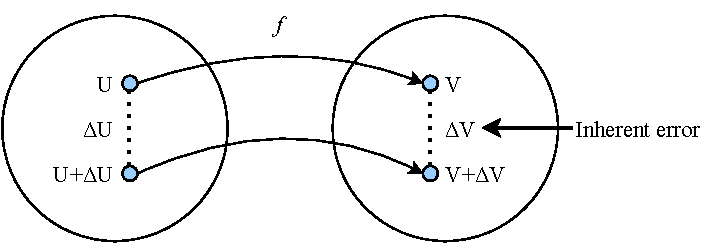
\includegraphics[width=0.6\textwidth]{img/_inherent_error.pdf}
            \caption{Inherent error visualization}
        \end{figure}
\end{description}



\section{Error measurement}

Let $x$ be a value and $\hat{x}$ its approximation. Then:
\begin{descriptionlist}
    \item[Absolute error] 
        \[
            E_{a} = \hat{x} - x 
            \marginnote{Absolute error}
        \] 
        Note that, out of context, the absolute error is meaningless.
    \item[Relative error] 
        \[
            E_{r} = \frac{\hat{x} - x}{x} 
            \marginnote{Relative error}
        \] 
\end{descriptionlist}



\section{Representation in base \texorpdfstring{$\beta$}{B}}

Let $\beta \in \mathbb{N}_{> 1}$ be the base.
Each $x \in \mathbb{R} \smallsetminus \{0\}$ can be uniquely represented as:
\begin{equation}
    \label{eq:finnum_b_representation}
    x = \texttt{sign}(x) \cdot (d_1\beta^{-1} + d_2\beta^{-2} + \dots + d_n\beta^{-n})\beta^p
\end{equation}
where:
\begin{itemize}
    \item $0 \leq d_i \leq \beta-1$
    \item $d_1 \neq 0$
    \item starting from an index $i$, not all $d_j$ ($j \geq i$) are equal to $\beta-1$
\end{itemize}
%
\Cref{eq:finnum_b_representation} can be represented using the normalized scientific notation as: \marginnote{Normalized scientific notation}
\[
    x = \pm (0.d_1d_2\dots) \beta^p
\]
where $0.d_1d_2\dots$ is the \textbf{mantissa} and $\beta^p$ the \textbf{exponent}. \marginnote{Mantissa\\Exponent}



\section{Floating-point}
A floating-point system $\mathcal{F}(\beta, t, L, U)$ is defined by the parameters: \marginnote{Floating-point}
\begin{itemize}
    \item $\beta$: base
    \item $t$: precision (number of digits in the mantissa)
    \item $[L, U]$: range of the exponent
\end{itemize}

Each $x \in \mathcal{F}(\beta, t, L, U)$ can be represented in its normalized form:
\begin{eqnarray}
    x = \pm (0.d_1d_2 \dots d_t) \beta^p & L \leq p \leq U
\end{eqnarray}
We denote with $\texttt{fl}(x)$ the representation of $x \in \mathbb{R}$ in a given floating-point system.

\begin{example}
    In $\mathcal{F}(10, 5, -3, 3)$, $x=12.\bar{3}$ is represented as:
    \begin{equation*}
        \texttt{fl}(x) = + 0.12333 \cdot 10^2
    \end{equation*}
\end{example}


\subsection{Numbers distribution}
Given a floating-point system $\mathcal{F}(\beta, t, L, U)$, the total amount of representable numbers is:
\begin{equation*}
    2(\beta-1) \beta^{t-1} (U-L+1)+1
\end{equation*}
%
Representable numbers are more sparse towards the exponent upper bound and more dense towards the lower bound.
It must be noted that there is an underflow area around 0.
\begin{figure}[H]
    \centering
    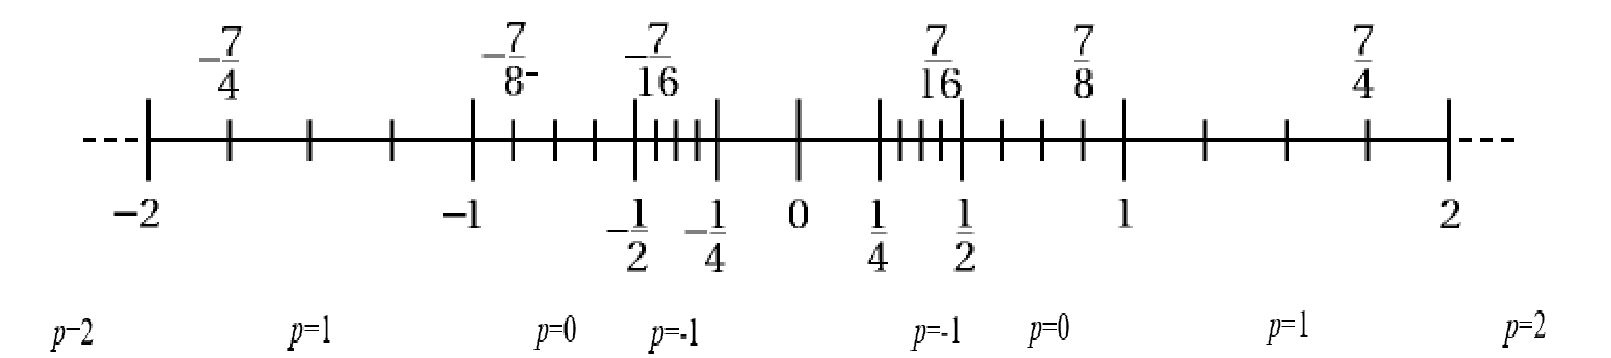
\includegraphics[width=0.8\textwidth]{img/floatingpoint_range.png}
    \caption{Floating-point numbers in $\mathcal{F}(2, 3, -1, 2)$}
\end{figure}


\subsection{Number representation}
Given a floating-point system $\mathcal{F}(\beta, t, L, U)$, the representation of $x \in \mathbb{R}$ can result in:
\begin{descriptionlist}
    \item[Exact representation] 
        if $p \in [L, U]$ and $d_i=0$ for $i>t$.

    \item[Approximation] \marginnote{Truncation\\Rounding}
        if $p \in [L, U]$ but $d_i$ may not be 0 for $i>t$. 
        In this case, the representation is obtained by truncating or rounding the value.

    \item[Underflow] \marginnote{Underflow}
        if $p < L$. In this case, the value is approximated to 0.

    \item[Overflow] \marginnote{Overflow}
        if $p > U$. In this case, an exception is usually raised.
\end{descriptionlist}


\subsection{Machine precision}
Machine precision $\varepsilon_{\text{mach}}$ determines the accuracy of a floating-point system. \marginnote{Machine precision}
Depending on the approximation approach, machine precision can be computed as:
\begin{descriptionlist}
    \item[Truncation] $\varepsilon_{\text{mach}} = \beta^{1-t}$
    \item[Rounding] $\varepsilon_{\text{mach}} = \frac{1}{2}\beta^{1-t}$
\end{descriptionlist}
Therefore, rounding results in more accurate representations.

$\varepsilon_{\text{mach}}$ is the smallest distance among the representable numbers (\Cref{fig:finnum_eps}).
\begin{figure}[H]
    \centering
    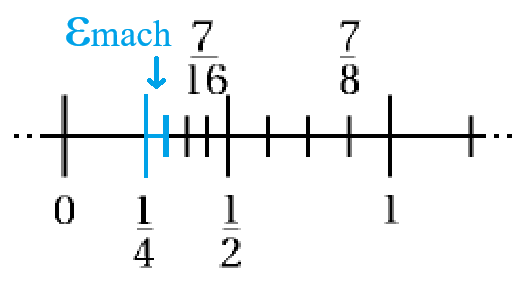
\includegraphics[width=0.2\textwidth]{img/machine_eps.png}
    \caption{Visualization of $\varepsilon_{\text{mach}}$ in $\mathcal{F}(2, 3, -1, 2)$}
    \label{fig:finnum_eps}
\end{figure}

In alternative, $\varepsilon_{\text{mach}}$ can be defined as the smallest representable number such that:
\begin{equation*}
    \texttt{fl}(1 + \varepsilon_{\text{mach}}) > 1.
\end{equation*}


\subsection{IEEE standard}
IEEE 754 defines two floating-point formats:
\begin{descriptionlist}
    \item[Single precision] Stored in 32 bits. Represents the system $\mathcal{F}(2, 24, -128, 127)$. \marginnote{\texttt{float32}}
        \begin{center}
            \small
            \begin{tabular}{|c|c|c|}
                \hline
                1 (sign) & 8 (exponent) & 23 (mantissa) \\
                \hline
            \end{tabular}
        \end{center}

    \item[Double precision] Stored in 64 bits. Represents the system $\mathcal{F}(2, 53, -1024, 1023)$. \marginnote{\texttt{float64}}
        \begin{center}
            \small
            \begin{tabular}{|c|c|c|}
                \hline
                1 (sign) & 11 (exponent) & 52 (mantissa) \\
                \hline
            \end{tabular}
        \end{center}
\end{descriptionlist}
As the first digit of the mantissa is always 1, it does not need to be stored.
Moreover, special configurations are reserved to represent \texttt{Inf} and \texttt{NaN}.


\subsection{Floating-point arithmetic}
Let:
\begin{itemize}
    \item $+: \mathbb{R} \times \mathbb{R} \rightarrow \mathbb{R}$ be a real numbers operation.
    \item $\oplus: \mathcal{F} \times \mathcal{F} \rightarrow \mathcal{F}$ be the corresponding operation in a floating-point system.
\end{itemize}
%
To compute $x \oplus y$, a machine:
\begin{enumerate}
    \item Calculates $x + y$ in a high precision register 
        (still approximated, but more precise than the floating-point system used to store the result)
    \item Stores the result as $\texttt{fl}(x + y)$
\end{enumerate}

A floating-point operation causes a small rounding error:
\[
    \left\vert \frac{(x \oplus y) - (x + y)}{x+y} \right\vert < \varepsilon_{\text{mach}}
\]
%
However, some operations may be subject to the \textbf{cancellation} problem which causes information loss.
\marginnote{Cancellation}
\begin{example}
    Given $x = 1$ and $y = 1 \cdot 10^{-17}$, we want to compute $x + y$ in $\mathcal{F}(10, 16, U, L)$.
    It is assumed that $U$ and $L$ are sufficient for this example.
    \begin{equation*}
        \begin{split}
            z & = \texttt{fl}(x) + \texttt{fl}(y) \\
              & = 0.1 \cdot 10^1 + 0.1 \cdot 10^{-16} \\
              & = (0.1 + 0.\overbrace{0\dots0}^{\mathclap{16\text{ zeros}}}1) \cdot 10^1 \\
              & = 0.1\overbrace{0\dots0}^{\mathclap{15\text{ zeros}}}1 \cdot 10^1
        \end{split}
    \end{equation*}
    Then, we have that $\texttt{fl}(z) = 0.1\overbrace{0\dots0}^{\mathclap{15\text{ zeros}}} \cdot 10^1 = 1 = x$.
\end{example}